\chapter{Introduction to Qt and SQL Programming}
So far we have designed the detailed software architecture. Before starting module design and implementation we have to introduce Qt GUI programming and SQL programming.

\section{Qt GUI Programming}
Qt identifies itself as a cross-platform software development framework. It was originally designed for making graphic user interface applications. The Qt framework consists of the following main modules. As the name indicates, Qt Core is the core of the Qt framework. It defines QObject, the base class of all Qt objects. QObject provides lower-level infrastructure for the Qt Framework and applications.

\begin{table}[htbp]
\centering
\caption {Qt Modules} \label{tab:Qt Modules}
\begin{tabular}{ll}
\hline
Module & Description \\
\hline
Qt Core & Core non-graphical classes used by other modules. \\ 
Qt GUI & Base classes for graphical user interface (GUI) components. Includes OpenGL. \\
Qt Multimedia & Classes for audio, video, radio and camera functionality. \\
Qt Multimedia Widgets & Widget-based classes for implementing multimedia functionality. \\
Qt Network & Classes to make network programming easier and more portable. \\
Qt QML & Classes for QML and JavaScript languages. \\
Qt Quick & A declarative framework for building highly dynamic applications with custom user interfaces. \\
Qt Quick Controls & Provides lightweight QML types for creating performant user interfaces for desktop, embedded, and mobile devices. These types employ a simple styling architecture and are very efficient. \\
Qt Quick Dialogs & Types for creating and interacting with system dialogs from a Qt Quick application. \\
Qt Quick Layouts & Layouts are items that are used to arrange Qt Quick 2 based items in the user interface. \\
Qt Quick Test & A unit test framework for QML applications, where the test cases are written as JavaScript functions. \\
Qt SQL & Classes for database integration using SQL. \\
Qt Test & Classes for unit testing Qt applications and libraries. \\
Qt Widgets & Classes to extend Qt GUI with C++ widgets. \\
\hline
\end{tabular}
\end{table}

Special attention should be paid to the Signal and Slot mechanism supported by QObject. It is a powerful, friendly and intuitive alternative to the callback technique, and is the central feature of Qt. When an event occurs, a signal is emitted. The corresponding slots receive that signal and respond by executing a function. The signal and slot mechanism has three elements: the signal, the slot, and connection. They can be illustrated with the figure below.

\begin{figure}[htbp]
\centering
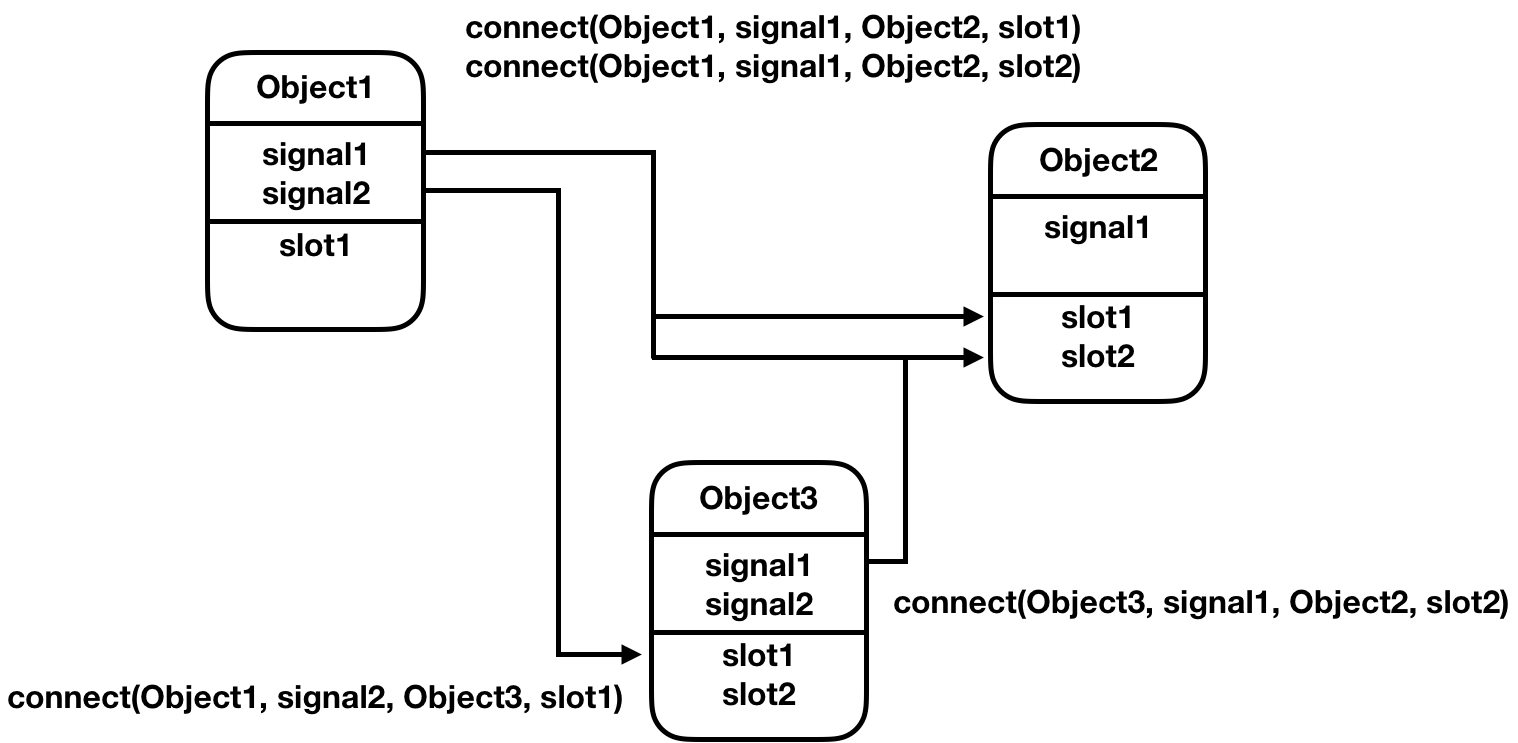
\includegraphics[width = \textwidth]{SignalAndSlot}
\caption{Signal and Slot\label{fig:Signal and Slot}}
\end{figure}

Qt has predefined many useful signals for the UI widgets, and they are automatically emitted once a corresponding even occurs. For example, when we click on a push button, it will send a click() signal. To customize the behavior of an event, we can define slot functions and connect them to the corresponding signal. We can also subclass the standard Qt widgets and define our own signal functions.

In a widget based application, Qt GUI and Qt Widgets must be included. Qt GUI classes provide infrastructure for user interfaces. They are extended to Qt Widgets, which are primary elements for creating GUI. Widgets can display data and status information, receive user input, and provide a container for other widgets that should be grouped together. Qt Widgets can be categorized into the following groups
\begin{itemize}
\item Layouts are geometry managers. They automatically arrange child widgets in their containers according to their sizeHint and sizePolicy properties. According to the direction in which child widgets are distributed, there are vertical, horizontal, grid and form layout.
\item Spacers provide blank space in a layout. There are vertical and horizontal spacer.
\item Buttons provide push button or checkable button widgets, among which the most frequently used are push buttons, check boxes and radio buttons. A special case is the button box, which contains a set of predefined push buttons and the buttons can be configured.
\item Item widgets/item views provide architecture to manage the relationship between data and the way it is presented to the user. There are list, tree, table view/widget etc.
\item Containers provide an area to group widgets together. There are group box, tool box, tab widget, stacked widget etc.
\item Input widgets provide a friendly way to take different types of user input. There are combo boxes, line edit, text edit, spin box etc. These text widgets can also be configured as readonly and used to display text data. Qt also provides widget to take date and/or time.
\item Display widgets provide a friendly way to display different types of data. There are labels, text browsers, calendar widgets, progress bars and so on.
\end{itemize}

Most of these basic widgets are configurable according to our requirements. We can also customize the widgets by subclassing them. With these widgets, we are able to make a strong and friendly user interface.

The Qt Company develops an IDE called Qt Creator. It is different from any other IDEs in that it is highly customized for Qt. It provides a very friendly and convenient wizard for creating Qt applications and what it calls designer form classes, which are essentially subclasses of Qt widgets such as QDialog, QMainWindow etc or the generic QWidget, depending on what kind of UI we want to create. The UI components are generated from the XML UI form and is a member variable of the designer form class;

\begin{lstlisting}[language=C++]
// designer form class header  
#include <QMainWindow>

namespace Ui {
class MainWindow;
}

class MainWindow : public QMainWindow
{
    Q_OBJECT
public:
    explicit MainWindow(QWidget *parent = nullptr);
    ~MainWindow();
private:
    Ui::MainWindow *ui; // instance of the UI class.
};
\end{lstlisting}

\begin{lstlisting}[language=C++]
// designer form class source code  
#include "mainwindow.h"
// header generated by Qt Creator.
// The UI class is defined here
#include "ui_mainwindow.h"  

MainWindow::MainWindow(QWidget *parent) :
    QMainWindow(parent),
    ui(new Ui::MainWindow)
{
    ui->setupUi(this);
}

MainWindow::~MainWindow()
{
    delete ui;
}
\end{lstlisting}

\section{SQL Programming}
In the chapter Section of Infrastructure, we have already introduced the relation database management systems and had some basic knowledge about them. We selected MySQL as our database system. Before starting implementation, we have to learn the SQL operations, the MySQL connector and the designed database structure.

\subsection{Database Operations}
1. Create, delete and select a database
\begin{lstlisting}[language=SQL]
CREATE DATABASE database_name;
USE DATABASE;
DROP DATABASE database_name;
\end{lstlisting}

2. Create and delete a table
\begin{lstlisting}[language=SQL]
CREATE TABLE table_name (column_name data_type);
DROP TABLE table_name ;
\end{lstlisting}

Example:
\begin{lstlisting}[language=SQL]
CREATE TABLE IF NOT EXISTS example_table (
   user_id INT AUTO_INCREMENT,
   name VARCHAR(100) NOT NULL,
   phone_number VARCHAR(40) NOT NULL,
   address DATE,
   PRIMARY KEY ( user_id )
) ENGINE=InnoDB DEFAULT CHARSET=utf8;
\end{lstlisting}

Special notes
AUTO\_INCREMENT: to make the integer increment by 1 automatically. Usually applied to primary keys.
NOT NULL: to force the data field to be not null.
PRIMARY KEY: to set the data field to be the primary key for indexing data rows.
ENGINE: to set the database engine.
CHARSET: to set character set for this table.

3. Alter a table
We can alter a table after it is created. With the ALTER TABLE statement, we are able to add a new column, drop an existing column, change a column’s name and its data type, change the table name, add keys and so on.

\begin{lstlisting}[language=SQL]
ALTER TABLE table_name  DROP column_name; -- to drop a column
ALTER TABLE table_name ADD column_name column_type [AFTER column_name_2]; -- to add a column [after another column]
ALTER TABLE table_name CHANGE column_name new_column_name column_type; -- to change the column name and type
ALTER TABLE table_name RENAME TO new_table_name; -- to change the table name
\end{lstlisting}

4. Add or drop a unique, primary and foreign key
To add a unique key, primary key or a foreign key, we apply a constraint to the table. Take the unique key for example. If a column is a unique key, then values of this column must be unique. Inserting a value which already exists in the table will fail. We can also add a unique key to multiple columns. In this case, the combination of values corresponding to the columns must be unique. A primary key is a unique key and must be not null. Each table can have at most one primary key. A foreign key is a field in table1 that refers to the primary key in table2. Value of this filed in table1 must exist in table2. These keys can be added upon creation of the table, or by ALTER TABLE statement afterwards.

\begin{lstlisting}[language=SQL]
ALTER TABLE table_name ADD UNIQUE (column_name);
ALTER TABLE table_name ADD UNIQUE (column1, column2, ..., columnN);
ALTER TABLE table_name ADD PRIMARY KEY (column_name);
ALTER TABLE table_name ADD PRIMARY KEY (column1, column2, ..., columnN);
ALTER TABLE table1 ADD FOREIGN KEY (column1) REFERENCES table2 (column2);
ALTER TABLE table_name DROP INDEX index_name;
ALTER TABLE table_name DROP PRIMARY KEY;
ALTER TABLE table_name DROP FOREIGN KEY index_name;
\end{lstlisting}

5. Insert, update and delete data
\begin{lstlisting}[language=SQL]
INSERT INTO table_name ( column1, column2,...columnN ) VALUES ( value1, value2,...valueN );
UPDATE table_name SET column1=new_value1, column2=new_value2 [WHERE conditions];
DELETE FROM table_name [WHERE conditions];
\end{lstlisting}

WHERE: to specify conditions. In practice, every table usually has a ID column, which is an AUTO\_INCREMENT primary key. If we know the value, we can do something like
\begin{lstlisting}[language=SQL]
DELETE FROM example_table WHERE user_id = "1";
\end{lstlisting}

6. Query data
\begin{lstlisting}[language=SQL]
SELECT field1, field2... FROM table_name [WHERE conditions];
SELECT * FROM table_name [WHERE conditions]; -- select all columns
\end{lstlisting}

The data fields to select can not only be a column of the data, but also a function. For example, we can count rows of the table by
\begin{lstlisting}[language=SQL]
SELECT COUNT(*) FROM table_name; 
\end{lstlisting}

In many cases we might want to select data from multiple related tables. We use the INNER JOIN key word as follows.
\begin{lstlisting}[language=SQL]
SELECT table1.field1, table1.field2, table2.field1 FROM table1, table2 WHERE table1.field_a = table2.field_b;
\end{lstlisting}
In such use cases, fielda of table1 usually references fieldb of table2 as a foreign key, or the other way around.

\subsection{Database Connector and Database Handler}
The MySQL uses the client/server architecture. Although we are able to connect to the server either by GUI tools such as MySQL Workbench or with command lines, to build a database application we have to use the MySQL Connector. MySQL Connector is not a standard component of the MySQL package. It can be downloaded from MySQL website and installed easily.

To use the connector, we need to include the header files in our code and initialize the database connection. First, we should create a driver instance, and connect it to the database server given the host name, username and password. Then, we will create a statement instance. To execute a query statement, call the executeQuery() function, and parse the result set. To execute any statement that writes the database, call the executeUpdate() function.

We realized that the raw APIs offered by the MySQL Connector is not so friendly and reusable. One problem is that we have to write a complete SQL statement for each query or update. This is not really necessary, because the statement is highly structured. We can write functions that accept only keywords, such as table name, column name, and generate complete statements. In this way, the API would be much more friendly to users. Another problem is that we have to manually parse the results for each query. Also, we can write a function to do this. Besides these, from an object-oriented programming point of view, it would be nice to wrap all these stuffs, the driver, the connection, statement and so on, in a class. So we designed a database handler class as below. In the code below we omit the database operation functions such as creating a table, querying data and so on.

\begin{lstlisting}[language=C++]
// database handler header
class DataBaseHandler
{
public:
    static bool initialize(const QString& hostname, const QString& database, const QString& username, const QString& password);
    static bool use_database(const QString &database);
    static void close();
    static void commit();
    static void rollback();

    /*
     We define database operation functions here.
    */

    static bool get_next_auto_increment_id(const QString& tablename, 
                                     const QString& id_field, 
                                     QString& id);
    static QString get_error_message();

private:
    static bool execute(const QString &statement);
    static bool execute_query(const QString &statement);

    static QString error_message_;
    static QString database_;
    static sql::Driver* driver_;
    static std::unique_ptr< sql::Connection > con_;
    static std::unique_ptr< sql::Statement > stmt_;
    static std::unique_ptr< sql::ResultSet > res_;
};
\end{lstlisting}

\begin{lstlisting}[language=C++]
// database handler source code
bool DataBaseHandler::initialize(const QString &hostname, const QString &database, const QString& username, const QString& password)
{
    try {
        con_.reset(driver_->connect(hostname.toUtf8().constData(),
            username.toUtf8().constData(),
            password.toUtf8().constData()));
        con_->setAutoCommit(false);
        if (database != "")
        {
            con_->setSchema(database.toUtf8().constData());
            database_ = database;
        }
        stmt_.reset(con_->createStatement());
        return true;
    } catch (sql::SQLException &e) {
        error_message_ = e.what();
        return false;
    }
}

bool DataBaseHandler::execute(const QString &statement)
{
    try {
        stmt_->executeUpdate(statement.toUtf8().constData());
        return true;
    } catch (sql::SQLException &e) {
        error_message_ = e.what();
      return false;
    }
}

bool DataBaseHandler::execute_query(const QString &statement)
{
    try {
        res_.reset(stmt_->executeQuery(statement.toUtf8().constData()));
        return true;
    } catch (sql::SQLException &e) {
        error_message_ = e.what();
      return false;
    }
}
\end{lstlisting}

This initialization of the database connection is wrapped in the initialize() function. After initialization, we can do database operations. Every database operation function parses its parameters and generate a SQL statement string, and either calls the execute() or the execute\_query() function, depending on whether it is to update or query the database. The return type of the database operation functions should always be bool so that we know whether they are successful. In practice we want to execute a series of SQL operations as a work unit which we call a transaction. One property of the transaction is atomicity. It requires that all SQL operations must be successful, or we have to move back to the point before this transaction. After each transaction we have to determine whether the conjunction of returned values are true, and commit() the transaction or rollback(). If a transaction failed, we can get the error message using the get\_error\_message() function.

\begin{lstlisting}[language=C++]
// database transaction example
bool success = true;
success = success && DataBaseHandler::some_operation();
success = success && DataBaseHandler::another_operation();
if (success) DataBaseHandler::commit();
else
{
    DataBaseHandler::rollback();
    QString error_message = DataBaseHandler::get_error_message();
    // do something
}
\end{lstlisting}

It’s to be noted that all member variables and functions inside the DataBaseHandler class are static. This is because the DataBaseHandler is very frequently used. We found it would be very inefficient if we create a DataBaseHandler instance, initialize the database connector every time we want to access the database. To make everything static, we only have to initialize the database connector and connect to the database server once, and the same connector instance is used every time and everywhere. We must initialize the database connector upon initialization of the software.

\section{Database Design}
Based on an existing draft, we designed the database structure consisting of a number of tables. The tables, data fields and types of each table and relationships between tables have be been illustrated in the diagram. 

\begin{figure}[htbp]
\centering
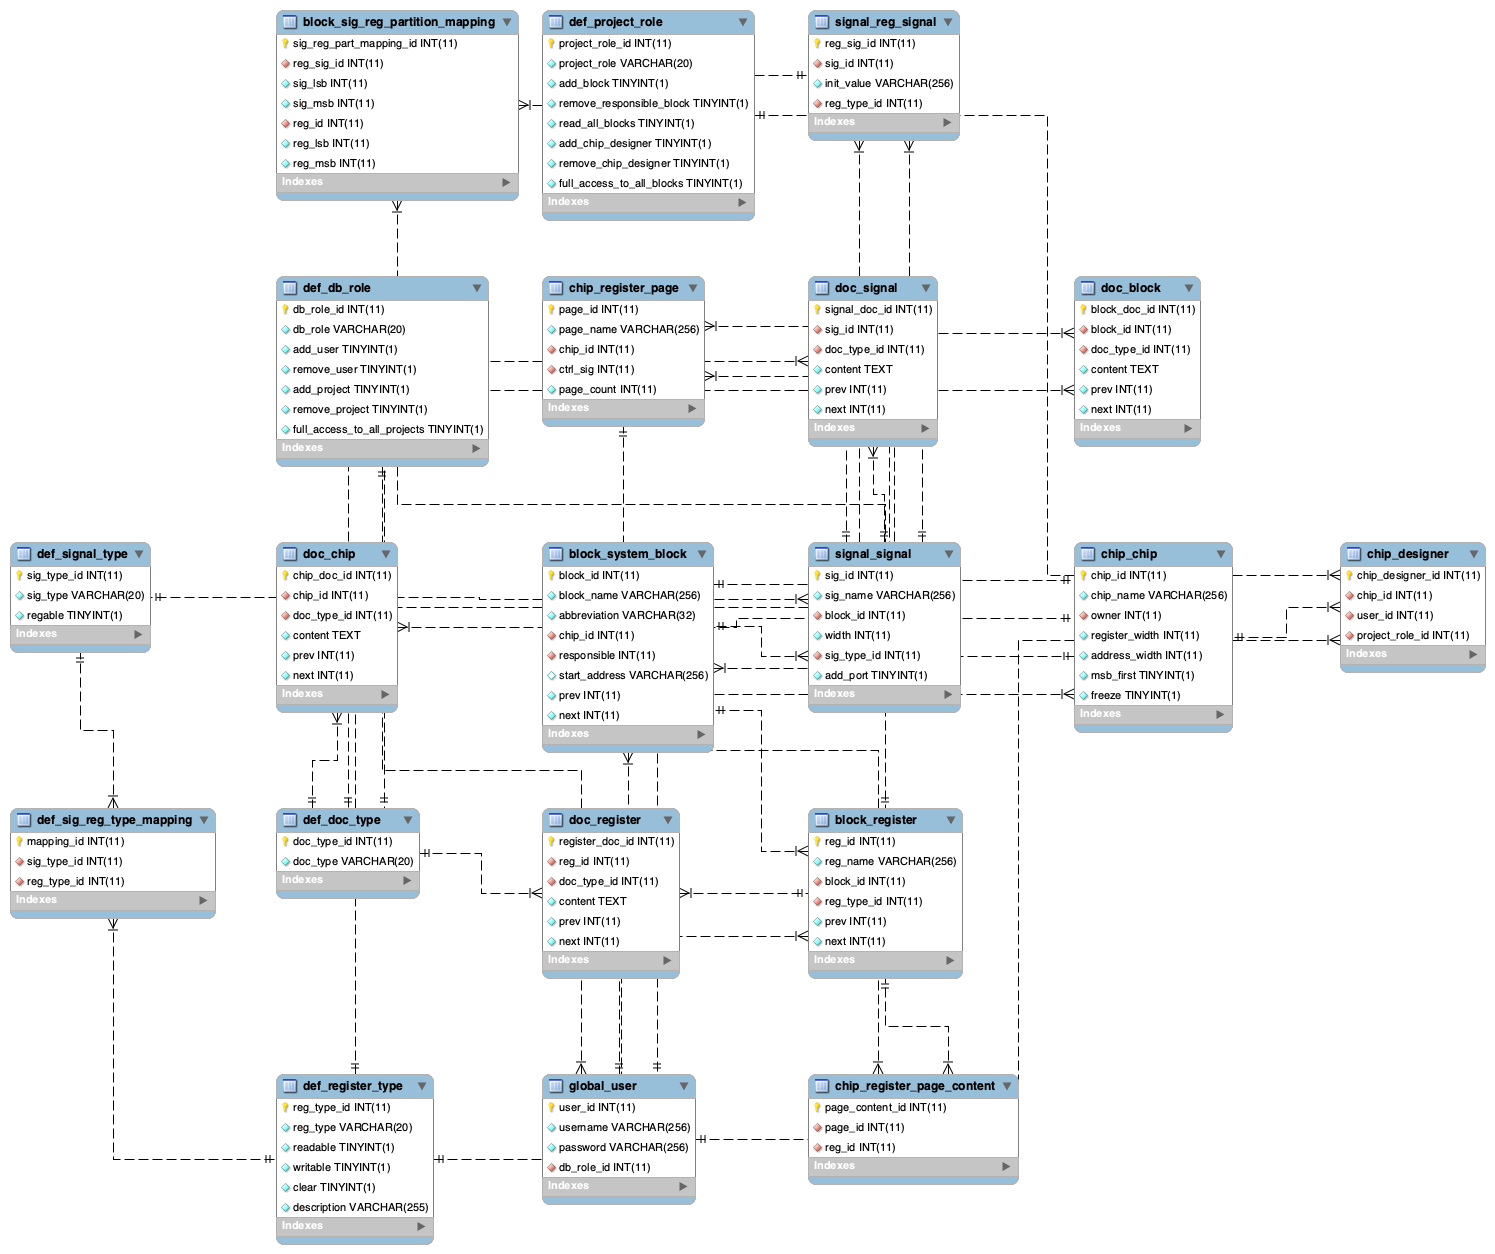
\includegraphics[width = \textwidth]{database}
\caption{Database Structure\label{fig:Database Structure}}
\end{figure}

The definitions of each database table is listed below. It;s to be noted that we do not hardcode e.g. project roles and register types in the software. Instead, they are defined in the tables starting with def and this provides us much flexibility. For example, we can add a new project role by simply adding a new row to the def\_project\_role table without modifying the software itself.

\begin{table}[htbp]
\centering
\caption {Database Table Definitions} \label{tab:Database Table Definitions}
\begin{tabular}{ll}
\hline
Table & Description \\
\hline
def\_sig\_reg\_type\_mapping & Pair of register types and signal types of which the signals and registers can be mapped to each other \\
def\_doc\_type & Definition of document types \\
global\_users & Users of the software \\
chip\_chip & Chips \\
chip\_designer & Designers of each chip \\
chip\_register\_page & Register pages of each chip \\
chip\_register\_page\_content & Registers for each register page \\
block\_system\_block & System blocks of each chip \\
block\_register & Register of each system block \\
block\_sig\_reg\_partition\_mapping & Mappings of signal and register partitions \\
signal\_signal & Signals of each system block \\
signal\_reg\_signal & Register signals for each signals that can be mapped to a register \\
doc\_chip & Chip level documents \\
doc\_block & System block level documents \\
doc\_register & Register level documents \\
doc\_signal & Signal level documents \\
\hline
\end{tabular}
\end{table}